
          %---------%
\chapter{~~Remeshing}\label{\numb section 10}
          %---------%

This section is devoted to remeshing algorithms.
Before proceeding please make sure you have read and understood paragraphs
\ref{\numb section 9.\numb parag 8} and \ref{\numb section 9.\numb parag 9}.


          %---------------------------------%
\section{~~Cutting a square along a diagonal}\label{\numb section 10.\numb parag 1}
          %---------------------------------%

Suppose we have a mesh of squares and for some reason we want to transform one of the
squares in two triangles, cutting it along one of its diagonals.

One way to achieve this is

\begin{Verbatim}[commandchars=\\\{\},formatcom=\small\tt,frame=single,
   label=parag-\ref{\numb section 10.\numb parag 1}.cpp,rulecolor=\color{coment},
   baselinestretch=0.94,framesep=2mm]
   ABCD.remove_from_mesh ( msh );
   \verm{Cell} \azul{AC} ( \verm{tag}::segment, A.reverse(), C );
   \verm{Cell} \azul{ABC} ( \verm{tag}::triangle, AB, BC, AC.reverse() );
   \verm{Cell} \azul{CDA} ( \verm{tag}::triangle, CD, DA, AC );
   ABC.add_to_mesh ( msh );
   CDA.add_to_mesh ( msh );
\end{Verbatim}

\begin{figure}[ht] \centering
  \psfrag{A}{\tt\textcolor{textindraw}{A}}
  \psfrag{B}{\tt\textcolor{textindraw}{B}}
  \psfrag{C}{\tt\textcolor{textindraw}{C}}
  \psfrag{D}{\tt\textcolor{textindraw}{D}}
  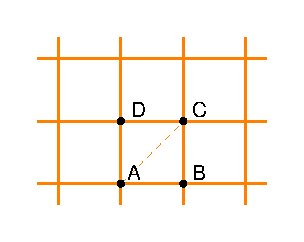
\includegraphics[width=50mm]{malha-quadr}
  \caption{A (part of a) mesh of squares}
  \label{\numb section 10.\numb fig 1}
\end{figure}

The only delicate point here is that the core of the {\small\tt\verm{Cell}} object
{\small\tt ABCD}
will become unused (and inaccessible when the wrapper goes out of syntactic scope).
If you have the garbage collector on (see paragraph \ref{\numb section 11.\numb parag 5}),
the core will be destroyed when the wrapper goes out of scope.
Otherwise, the core will continue to occupy space in the computer's memory giving rise
to an undesirable phenomenon known as ``memory leak''.
If your program does this a lot, it will occupy increasingly more memory without reason.


                 %-------------------------------------%
\section{~~\cinza{Transforming a square into a triangle}}\label{\numb section 10.\numb parag 2}
                 %-------------------------------------%

{\normalfont\bfseries The code described in this paragraph does not work.
The internal representation of {\small\tt Mesh::Connected::OneDim} requires a different
implementation of methods {\small\tt add\_\,to\_\,mesh}, {\small\tt remove\_\,from\_\,mesh},
{\small\tt glue\_\,on\_\,bdry\_\,of} and {\small\tt cut\_\,from\_\,bdry\_\,of}.              }

Instead of discarding the square and building two new triangles, we can use the same
{\small\tt\verm{Cell}} object {\small\tt ABCD}
by transforming it into a triangle, without removing it from {\small\tt msh}, then add
a new triangle to obtain the same result as in paragraph \ref{\numb section 10.\numb parag 1}.

\begin{Verbatim}[commandchars=\\\{\},formatcom=\small\tt,frame=single,
   label=parag-\ref{\numb section 10.\numb parag 2}.cpp,rulecolor=\color{coment},
   baselinestretch=0.94,framesep=2mm]
   CD.cut_from_bdry_of ( ABCD );
   DA.cut_from_bdry_of ( ABCD );
   \cinza{// at this point, ABCD is a cell whose boundary is incomplete}
   \cinza{// it has only two sides and an opening}
   \cinza{// however, it still is part of 'msh'}
   \verm{Cell} \azul{AC} ( \verm{tag}::segment, A.reverse(), C );
   AC.reverse().glue_on_bdry_of ( ABCD );
   \cinza{// at this point, and in spite of its name, ABCD is no longer a square}
   \cinza{// it is a triangle, still part of 'msh'}
   \verm{Cell} \azul{CDA} ( \verm{tag}::triangle, CD, DA, AC );
   CDA.add_to_mesh ( msh );
\end{Verbatim}



          %--------------------------------%
\section{~~Modifying the mesh within a loop}\label{\numb section 10.\numb parag 3}
          %--------------------------------%

As is the case with many {\tt C++} containers, it is not safe to modify a mesh while
iterating over its cells.
For instance, code below gives undefined behaviour (often, a {\small\tt segmentation fault}
will occur).

\begin{Verbatim}[commandchars=\\\{\},formatcom=\small\tt,frame=single,
   label=incorrect code !,rulecolor=\color{coment},
   baselinestretch=0.94,framesep=2mm]
   \verm{CellIterator} \azul{it} = msh.iterator ( \verm{tag}::over_cells_of_dim, 2 );
   for ( it.reset(); it.in_range(); it++ )
   \{  \verm{Cell} \azul{square} = *it;
      if ( \cinza{... some criterion ...} )
      \{  square.remove_from_mesh ( msh );
         \cinza{// statement above opens the path to disaster}
         \cinza{// next time 'it' is incremented, we get undefined behaviour}
         \cinza{// we may add other cells afterwards, at no good}
         some_other_cell.add_to_mesh ( msh );     \}   \}
\end{Verbatim}

You can circumvent this problem by creating a list of cells to be eliminated.
In the code below, we actually use two lists, one of squares, the other of vertices within
the boundary of those squares.
The vertices give an indication about which diagonal to choose to cut the square.

\begin{Verbatim}[commandchars=\\\{\},formatcom=\small\tt,frame=single,
   label=parag-\ref{\numb section 10.\numb parag 3}.cpp,rulecolor=\color{coment},
   baselinestretch=0.94,framesep=2mm]
   std::list<\verm{Cell}> list_of_squares, list_of_vertices;
   \verm{CellIterator} \azul{it} = msh.iterator ( \verm{tag}::over_cells_of_dim, 2 );
   for ( it.reset(); it.in_range(); it++ )
   \{  \verm{Cell} \azul{square} = *it;
      if ( \cinza{... some criterion ...} )  \cinza{// we decide to cut this square in halves}
      \{  list_of_squares.push_back ( square );
         \cinza{// according to some other criterion,}
         \cinza{// we choose a vertex and cut the square along this diagonal}
         \verm{Cell} \azul{P} = \cinza{...};  
         list_of_vertices.push_back ( P );       \}   \}

   assert ( list_of_squares.size() == list_of_vertices.size() );
   for ( std::list<\verm{Cell}>::iterator \azul{it1} = list_of_squares.begin(),
                                   \azul{it2} = list_of_vertices.begin();
         it1 != list_of_squares.end(); it1++, it2++                )
   \{  assert ( it2 != list_of_vertices.end() );
      \verm{Cell} \azul{square} = *it1, P = *it2;
      \verm{Cell} \azul{PQ} = square.boundary().cell_in_front_of ( P );
      \verm{Cell} \azul{Q} = PQ.tip();
      \verm{Cell} \azul{QR} = square.boundary().cell_in_front_of ( Q );
      \verm{Cell} \azul{R} = QR.tip();
      \verm{Cell} \azul{RS} = square.boundary().cell_in_front_of ( R );
      \verm{Cell} \azul{S} = RS.tip();
      \verm{Cell} \azul{SP} = square.boundary().cell_in_front_of ( S );
      assert ( SP.tip() == P );
      square.remove_from_mesh ( msh );
      \verm{Cell} \azul{PR} ( \verm{tag}::segment, P.reverse(), R );
      \verm{Cell} \azul{PQR} ( \verm{tag}::triangle, PQ, QR, PR.reverse() );
      PQR.add_to_mesh ( msh );
      \verm{Cell} \azul{RSP} ( \verm{tag}::triangle, RS, SP, PR );
      RSP.add_to_mesh ( msh );                                     \}
\end{Verbatim}
